\chapter{Design} 
\thispagestyle{plain} 
A key problem to solve with real-time computation is how to manage state so that updates are idempotent in the face of failures and retries. It's impossible to eliminate failures, so when a node dies or something else goes wrong, batches need to be retried. The question is - how do you do state updates (whether external databases or state internal to the topology) so that it's like each message was processed only once?
This is a tricky problem, and can be illustrated with the following example. Suppose that you're doing a count aggregation of your stream and want to store the running count in a database. If you store only the count in the database and it's time to apply a state update for a batch, there's no way to know if you applied that state update before. The batch could have been attempted before, succeeded in updating the database, and then failed at a later step. Or the batch could have been attempted before and failed to update the database. You just don't know.
Trident solves this problem by doing two things:\\[2mm]
1. Each batch is given a unique id called the 'transaction id'. If a batch is retried it will have the exact same transaction id.\\[2mm]
2. State updates are ordered among batches. That is, the state updates for batch 3 won't be applied until the state updates for batch 2 have succeeded.\\[2mm]
With these two primitives, you can achieve exactly-once semantics with your state updates. Rather than store just the count in the database, what you can do instead is store the transaction id with the count in the database as an atomic value. Then, when updating the count, you can just compare the transaction id in the database with the transaction id for the current batch. If they're the same, you skip the update - because of the strong ordering, you know for sure that the value in the database incorporates the current batch. If they're different, you increment the count.
Of course, you don't have to do this logic manually in your topologies. This logic is wrapped by the State abstraction and done automatically. Nor is your State object required to implement the transaction id trick: if you don't want to pay the cost of storing the transaction id in the database, you don't have to. In that case the State will have at-least-once-processing semantics in the case of failures (which may be fine for your application). You can read more about how to implement a State and the various fault-tolerance tradeoffs possible in this doc.
A State is allowed to use whatever strategy it wants to store state. So it could store state in an external database or it could keep the state in-memory but backed by HDFS (like how HBase works). States are not required to hold onto state forever. For example, you could have an in-memory State implementation that only keeps the last X hours of data available and drops anything older. Take a look at the implementation of the Memcached integration for an example State implementation.
\section{System Architecture}
\begin{center}
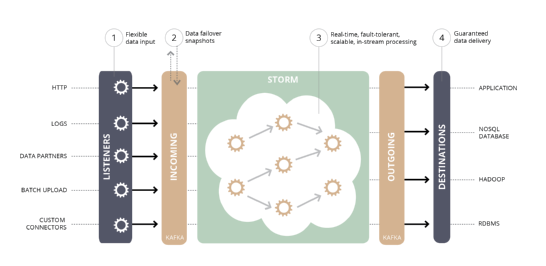
\includegraphics[scale=.7]{../img/img8} \\[2mm]
\end{center}
\subsection*{State in Trident}
Trident has first-class abstractions for reading from and writing to stateful sources. The state can either be internal to the topology - e.g., kept in-memory and backed by HDFS - or externally stored in a database like Memcached or Cassandra. There's no difference in the Trident API for either case.
Trident manages state in a fault-tolerant way so that state updates are idempotent in the face of retries and failures. This lets you reason about Trident topologies as if each message were processed exactly-once.There are various levels of fault-tolerance possible when doing state updates. Before getting to those, let's look at an example that illustrates the tricks necessary to achieve exactly-once semantics. Suppose that you're doing a count aggregation of your stream and want to store the running count in a database. Now suppose you store in the database a single value representing the count and every time you process a new tuple you increment the count.When failures occur, tuples will be replayed. This brings up a problem when doing state updates (or anything with side effects) - you have no idea if you've ever successfully updated the state based on this tuple before. Perhaps you never processed the tuple before, in which case you should increment the count. Perhaps you've processed the tuple and successfully incremented the count, but the tuple failed processing in another step. In this case, you should not increment the count. Or perhaps you saw the tuple before but got an error when updating the database. In this case, you should update the database.By just storing the count in the database, you have no idea whether or not this tuple has been processed before. So you need more information in order to make the right decision. Trident provides the following semantics which are sufficient for achieving exactly-once processing semantics:\\[2mm]
1. Tuples are processed as small batches\\[2mm]
2. Each batch of tuples is given a unique id called the "transaction id" (txid). If the batch is replayed, it is given the exact same txid.\\[2mm]
3. State updates are ordered among batches. That is, the state updates for batch 3 won't be applied until the state updates for batch 2 have succeeded.\\[2mm]
With these primitives, your State implementation can detect whether or not the batch of tuples has been processed before and take the appropriate action to update the state in a consistent way. The action you take depends on the exact semantics provided by your input spouts as to what's in each batch. There are three kinds of spouts possible with respect to fault-tolerance: "non-transactional", "transactional", and "opaque transactional". Likewise, there are three kinds of state possible with respect to fault-tolerance: "non-transactional", "transactional", and "opaque transactional". Let's take a look at each spout type and see what kind of fault-tolerance you can achieve with each.

\subsection*{Fault Tolerant Architecture} 
\begin{center}
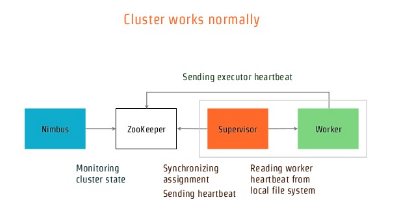
\includegraphics[scale=.7]{../img/img9} \\[2mm]
\end{center}
\begin{center}
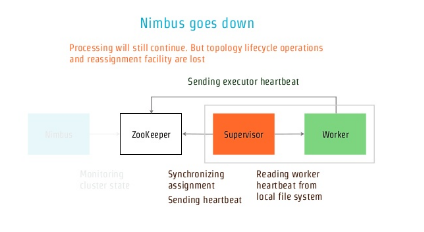
\includegraphics[scale=.7]{../img/img10} \\[2mm]
\end{center}
\begin{center}
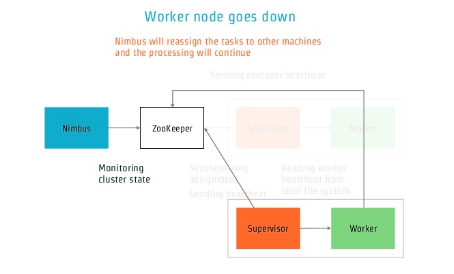
\includegraphics[scale=.7]{../img/img11} \\[2mm]
\end{center}
\begin{center}
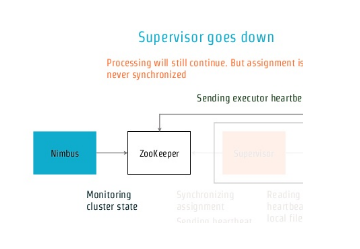
\includegraphics[scale=.7]{../img/img12} \\[2mm]
\end{center}

\section{State Diagram}
\subsection*{\normalsize Proposed system architecture}
\begin{center}
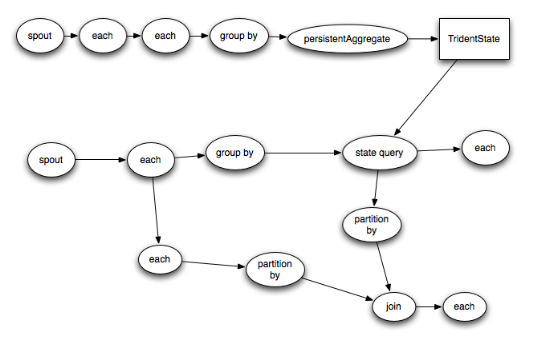
\includegraphics[scale=.7]{../img/img13} \\[2mm]
\end{center}
\begin{center}
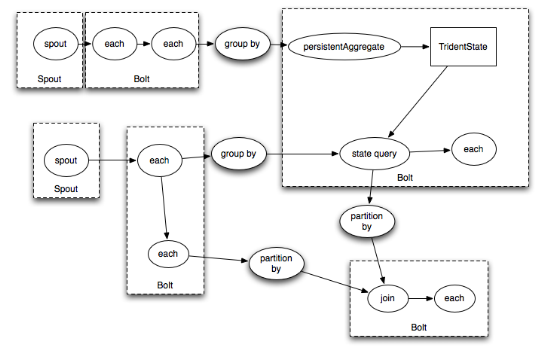
\includegraphics[scale=.7]{../img/img14} \\[2mm]
\end{center}

\section{Summary of spout and state types}
This diagram shows which combinations of spouts / states enable exactly-once messaging semantics:\\[2mm]
\begin{center}
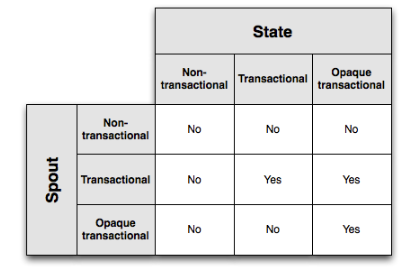
\includegraphics[scale=.7]{../img/img15} \\[2mm]
\end{center}
Opaque transactional states have the strongest fault-tolerance, but this comes at the cost of needing to store the txid and two values in the database. Transactional states require less state in the database, but only work with transactional spouts. Finally, non-transactional states require the least state in the database but cannot achieve exactly-once semantics.
The state and spout types you choose are a tradeoff between fault-tolerance and storage costs, and ultimately your application requirements will determine which combination is right for you.\\[2mm]
{\bfseries State APIs}\\[2mm]
You've seen the intricacies of what it takes to achieve exactly-once semantics. The nice thing about Trident is that it internalizes all the fault-tolerance logic within the State - as a user you don't have to deal with comparing txids, storing multiple values in the database, or anything like that. You can write code like this:\\[2mm]
\begin{verbatim}
TridentTopology topology = new TridentTopology();        
TridentState wordCounts =
      topology.newStream("spout1", spout)
        .each(new Fields("sentence"), new Split(), new Fields("word"))
        .groupBy(new Fields("word"))
        .persistentAggregate(MemcachedState.opaque(serverLocations), new Count(), new Fields("count"))                
        .parallelismHint(6);
\end{verbatim}
All the logic necessary to manage opaque transactional state logic is internalized in the MemcachedState.opaque call. Additionally, updates are automatically batched to minimize roundtrips to the database.\\[2mm]
The base State interface just has two methods:\\[2mm]
\begin{verbatim}
 public interface State {
    void beginCommit(Long txid); // can be null for things like partitionPersist occurring off a DRPC stream
    void commit(Long txid);
}
\end{verbatim}
You're told when a state update is beginning, when a state update is ending, and you're given the txid in each case. Trident assumes nothing about how your state works, what kind of methods there are to update it, and what kind of methods there are to read from it.\\[2mm]Suppose you have a home-grown database that contains user location information and you want to be able to access it from Trident. Your State implementation would have methods for getting and setting user information:\\[2mm]
\begin{verbatim}
 public class LocationDB implements State {
    public void beginCommit(Long txid) {    
    }
    
    public void commit(Long txid) {    
    }
    
    public void setLocation(long userId, String location) {
      // code to access database and set location
    }
    
    public String getLocation(long userId) {
      // code to get location from database
    }
}
\end{verbatim}
You then provide Trident a StateFactory that can create instances of your State object within Trident tasks. The StateFactory for your LocationDB might look something like this:\\[2mm]
\begin{verbatim}
public class LocationDBFactory implements StateFactory {
   public State makeState(Map conf, int partitionIndex, int numPartitions) {
      return new LocationDB();
   } 
}
\end{verbatim}
Trident provides the QueryFunction interface for writing Trident operations that query a source of state, and the StateUpdater interface for writing Trident operations that update a source of state. For example, let's write an operation "QueryLocation" that queries the LocationDB for the locations of users. Let's start off with how you would use it in a topology. Let's say this topology consumes an input stream of userids:\\[2mm]
\begin{verbatim}
TridentTopology topology = new TridentTopology();
TridentState locations = topology.newStaticState(new LocationDBFactory());
topology.newStream("myspout", spout)
        .stateQuery(locations, new Fields("userid"), new QueryLocation(), new Fields("location"))\\[2mm]
\end{verbatim}
Now let's take a look at what the implementation of QueryLocation would look like:\\[2mm]
\begin{verbatim}
public class QueryLocation extends BaseQueryFunction<LocationDB, String> {
    public List<String> batchRetrieve(LocationDB state, List<TridentTuple> inputs) {
        List<String> ret = new ArrayList();
        for(TridentTuple input: inputs) {
            ret.add(state.getLocation(input.getLong(0)));
        }
        return ret;
    }

    public void execute(TridentTuple tuple, String location, TridentCollector collector) {
        collector.emit(new Values(location));
    }    
}
\end{verbatim}
QueryFunction's execute in two steps. First, Trident collects a batch of reads together and passes them to batchRetrieve. In this case, batchRetrieve will receive multiple user ids. batchRetrieve is expected to return a list of results that's the same size as the list of input tuples. The first element of the result list corresponds to the result for the first input tuple, the second is the result for the second input tuple, and so on.You can see that this code doesn't take advantage of the batching that Trident does, since it just queries the LocationDB one at a time. So a better way to write the LocationDB would be like this:\\[2mm]
\begin{verbatim}
public class LocationDB implements State {
    public void beginCommit(Long txid) {    
    }
    public void commit(Long txid) {    
    }
    public void setLocationsBulk(List<Long> userIds, List<String> locations) {
      // set locations in bulk
    }
    public List<String> bulkGetLocations(List<Long> userIds) {
      // get locations in bulk
    }
}
\end{verbatim}
Then, you can write the QueryLocation function like this:\\[2mm]
\begin{verbatim}
public class QueryLocation extends BaseQueryFunction<LocationDB, String> {
    public List<String> batchRetrieve(LocationDB state, List<TridentTuple> inputs) {
        List<Long> userIds = new ArrayList<Long>();
        for(TridentTuple input: inputs) {
            userIds.add(input.getLong(0));
        }
        return state.bulkGetLocations(userIds);
    }

    public void execute(TridentTuple tuple, String location, TridentCollector collector) {
        collector.emit(new Values(location));
    }    
}
\end{verbatim}
This code will be much more efficient by reducing roundtrips to the database.
To update state, you make use of the StateUpdater interface. Here's a StateUpdater that updates a LocationDB with new location information:\\[2mm]
\begin{verbatim}
public class LocationUpdater extends BaseStateUpdater<LocationDB> {
    public void updateState(LocationDB state, List<TridentTuple> tuples, TridentCollector collector) {
        List<Long> ids = new ArrayList<Long>();
        List<String> locations = new ArrayList<String>();
        for(TridentTuple t: tuples) {
            ids.add(t.getLong(0));
            locations.add(t.getString(1));
        }
        state.setLocationsBulk(ids, locations);
    }
}
\end{verbatim}
Here's how you would use this operation in a Trident topology:\\[2mm]
\begin{verbatim}
TridentTopology topology = new TridentTopology();
TridentState locations = 
    topology.newStream("locations", locationsSpout)
        .partitionPersist(new LocationDBFactory(), new Fields("userid", "location"), new LocationUpdater())
\end{verbatim}
The partitionPersist operation updates a source of state. The StateUpdater receives the State and a batch of tuples with updates to that State. This code just grabs the userids and locations from the input tuples and does a bulk set into the State. partitionPersist returns a TridentState object representing the location db being updated by the Trident topology. You could then use this state in stateQuery operations elsewhere in the topology.You can also see that StateUpdaters are given a TridentCollector. Tuples emitted to this collector go to the "new values stream". In this case, there's nothing interesting to emit to that stream, but if you were doing something like updating counts in a database, you could emit the updated counts to that stream. You can then get access to the new values stream for further processing via the TridentState newValuesStream method.
